% Options for packages loaded elsewhere
\PassOptionsToPackage{unicode}{hyperref}
\PassOptionsToPackage{hyphens}{url}
\PassOptionsToPackage{dvipsnames,svgnames,x11names}{xcolor}
%
\documentclass[
  11pt,
]{article}

\usepackage{amsmath,amssymb}
\usepackage{iftex}
\ifPDFTeX
  \usepackage[T1]{fontenc}
  \usepackage[utf8]{inputenc}
  \usepackage{textcomp} % provide euro and other symbols
\else % if luatex or xetex
  \usepackage{unicode-math}
  \defaultfontfeatures{Scale=MatchLowercase}
  \defaultfontfeatures[\rmfamily]{Ligatures=TeX,Scale=1}
\fi
\usepackage{lmodern}
\ifPDFTeX\else  
    % xetex/luatex font selection
\fi
% Use upquote if available, for straight quotes in verbatim environments
\IfFileExists{upquote.sty}{\usepackage{upquote}}{}
\IfFileExists{microtype.sty}{% use microtype if available
  \usepackage[]{microtype}
  \UseMicrotypeSet[protrusion]{basicmath} % disable protrusion for tt fonts
}{}
\makeatletter
\@ifundefined{KOMAClassName}{% if non-KOMA class
  \IfFileExists{parskip.sty}{%
    \usepackage{parskip}
  }{% else
    \setlength{\parindent}{0pt}
    \setlength{\parskip}{6pt plus 2pt minus 1pt}}
}{% if KOMA class
  \KOMAoptions{parskip=half}}
\makeatother
\usepackage{xcolor}
\usepackage[lmargin=1in,rmargin=1in,tmargin=1in,bmargin=1in]{geometry}
\setlength{\emergencystretch}{3em} % prevent overfull lines
\setcounter{secnumdepth}{3}
% Make \paragraph and \subparagraph free-standing
\ifx\paragraph\undefined\else
  \let\oldparagraph\paragraph
  \renewcommand{\paragraph}[1]{\oldparagraph{#1}\mbox{}}
\fi
\ifx\subparagraph\undefined\else
  \let\oldsubparagraph\subparagraph
  \renewcommand{\subparagraph}[1]{\oldsubparagraph{#1}\mbox{}}
\fi


\providecommand{\tightlist}{%
  \setlength{\itemsep}{0pt}\setlength{\parskip}{0pt}}\usepackage{longtable,booktabs,array}
\usepackage{calc} % for calculating minipage widths
% Correct order of tables after \paragraph or \subparagraph
\usepackage{etoolbox}
\makeatletter
\patchcmd\longtable{\par}{\if@noskipsec\mbox{}\fi\par}{}{}
\makeatother
% Allow footnotes in longtable head/foot
\IfFileExists{footnotehyper.sty}{\usepackage{footnotehyper}}{\usepackage{footnote}}
\makesavenoteenv{longtable}
\usepackage{graphicx}
\makeatletter
\def\maxwidth{\ifdim\Gin@nat@width>\linewidth\linewidth\else\Gin@nat@width\fi}
\def\maxheight{\ifdim\Gin@nat@height>\textheight\textheight\else\Gin@nat@height\fi}
\makeatother
% Scale images if necessary, so that they will not overflow the page
% margins by default, and it is still possible to overwrite the defaults
% using explicit options in \includegraphics[width, height, ...]{}
\setkeys{Gin}{width=\maxwidth,height=\maxheight,keepaspectratio}
% Set default figure placement to htbp
\makeatletter
\def\fps@figure{htbp}
\makeatother
% definitions for citeproc citations
\NewDocumentCommand\citeproctext{}{}
\NewDocumentCommand\citeproc{mm}{%
  \begingroup\def\citeproctext{#2}\cite{#1}\endgroup}
\makeatletter
 % allow citations to break across lines
 \let\@cite@ofmt\@firstofone
 % avoid brackets around text for \cite:
 \def\@biblabel#1{}
 \def\@cite#1#2{{#1\if@tempswa , #2\fi}}
\makeatother
\newlength{\cslhangindent}
\setlength{\cslhangindent}{1.5em}
\newlength{\csllabelwidth}
\setlength{\csllabelwidth}{3em}
\newenvironment{CSLReferences}[2] % #1 hanging-indent, #2 entry-spacing
 {\begin{list}{}{%
  \setlength{\itemindent}{0pt}
  \setlength{\leftmargin}{0pt}
  \setlength{\parsep}{0pt}
  % turn on hanging indent if param 1 is 1
  \ifodd #1
   \setlength{\leftmargin}{\cslhangindent}
   \setlength{\itemindent}{-1\cslhangindent}
  \fi
  % set entry spacing
  \setlength{\itemsep}{#2\baselineskip}}}
 {\end{list}}
\usepackage{calc}
\newcommand{\CSLBlock}[1]{\hfill\break\parbox[t]{\linewidth}{\strut\ignorespaces#1\strut}}
\newcommand{\CSLLeftMargin}[1]{\parbox[t]{\csllabelwidth}{\strut#1\strut}}
\newcommand{\CSLRightInline}[1]{\parbox[t]{\linewidth - \csllabelwidth}{\strut#1\strut}}
\newcommand{\CSLIndent}[1]{\hspace{\cslhangindent}#1}

\makeatletter
\@ifpackageloaded{float}{}{\usepackage{float}}
\floatstyle{plain}
\@ifundefined{c@chapter}{\newfloat{atbl}{h}{loatbl}}{\newfloat{atbl}{h}{loatbl}[chapter]}
\floatname{atbl}{Table A}
\floatstyle{plaintop}
\restylefloat{atbl}
\newcommand*\quartoatblref[1]{Table \hyperref[#1]{A\ref{#1}}}
\@ifpackageloaded{caption}{}{\usepackage{caption}}
\DeclareCaptionLabelFormat{quartoatblreflabelformat}{#1#2}
\captionsetup[atbl]{labelformat=quartoatblreflabelformat}
\newcommand*\listofatbls{\listof{atbl}{List of Appendix Tabless}}
\makeatother
\makeatletter
\@ifpackageloaded{caption}{}{\usepackage{caption}}
\AtBeginDocument{%
\ifdefined\contentsname
  \renewcommand*\contentsname{Table of contents}
\else
  \newcommand\contentsname{Table of contents}
\fi
\ifdefined\listfigurename
  \renewcommand*\listfigurename{List of Figures}
\else
  \newcommand\listfigurename{List of Figures}
\fi
\ifdefined\listtablename
  \renewcommand*\listtablename{List of Tables}
\else
  \newcommand\listtablename{List of Tables}
\fi
\ifdefined\figurename
  \renewcommand*\figurename{Figure}
\else
  \newcommand\figurename{Figure}
\fi
\ifdefined\tablename
  \renewcommand*\tablename{Table}
\else
  \newcommand\tablename{Table}
\fi
}
\@ifpackageloaded{float}{}{\usepackage{float}}
\floatstyle{ruled}
\@ifundefined{c@chapter}{\newfloat{codelisting}{h}{lop}}{\newfloat{codelisting}{h}{lop}[chapter]}
\floatname{codelisting}{Listing}
\newcommand*\listoflistings{\listof{codelisting}{List of Listings}}
\makeatother
\makeatletter
\makeatother
\makeatletter
\@ifpackageloaded{caption}{}{\usepackage{caption}}
\@ifpackageloaded{subcaption}{}{\usepackage{subcaption}}
\makeatother
\ifLuaTeX
  \usepackage{selnolig}  % disable illegal ligatures
\fi
\usepackage{bookmark}

\IfFileExists{xurl.sty}{\usepackage{xurl}}{} % add URL line breaks if available
\urlstyle{same} % disable monospaced font for URLs
\hypersetup{
  pdftitle={The Hidden Poor: Solving Time Poverty through Redistribution of Household Production},
  pdfauthor={Fernando Rios-Avila; Aashima Sinha},
  pdfkeywords={Time Poverty, Income Poverty, Redistribution , household
production, care work, gender equality, LIMTIP},
  colorlinks=true,
  linkcolor={blue},
  filecolor={Maroon},
  citecolor={Blue},
  urlcolor={Blue},
  pdfcreator={LaTeX via pandoc}}


\usepackage{datetime}
\usepackage{booktabs}
\usepackage{chngcntr}
\usepackage{apptools}
\usepackage{lipsum}
\AtAppendix{\counterwithin{table}{section}}
\AtAppendix{\counterwithin{figure}{section}}

\title{The Hidden Poor: Solving Time Poverty through Redistribution of
Household Production}
\author{
Fernando Rios-Avila\\
Levy Economics Institute\\
\\
\and 
Aashima Sinha\\
Levy Economics Institute\\
\\
}
\date{2024-06-06}
\begin{document}


\def\spacingset#1{\renewcommand{\baselinestretch}%
{#1}\small\normalsize} \spacingset{1}

%Ipsum lorem

\maketitle
\begin{abstract}
\lipsum[1]
\end{abstract}
 
\vspace{.2in}

\textbf{\textit{Keyword: }}
    Time Poverty, Income Poverty, Redistribution , household production,
care work, gender equality, LIMTIP, 
    Time Poverty, Income Poverty, Redistribution , household production,
care work, gender equality, LIMTIP 


\thispagestyle{empty}
\clearpage\pagenumbering{arabic}
\newpage
\spacingset{1.2} % DON'T change the spacing!
\section{Introduction}\label{introduction}

Redistribution of household production has been identified as an
important tool to achieve gender equality (Elson The incorporation of
the 3R (recognizition, reduction adn redistribution) strategy as a
target in the sustainable development goals, is a testament to the
decades of activism and advocacy emphasizing that inequality on this
front cannot be justified in the name of ``private family matter''
rather is a matter of public policy.

While redistribution of household production responsibilities from women
to men is important intrsinsically for human rights and fairness
concerns, it is also instrumental in achieving gender equality in labor
market outcomes (Bruyn-Hundt, 1996; Elso, 2017; Esquivel, 2016). Studies
have demonstrated that gender gaps in the workforce and the unequal
sharing of household responsibilities can severely impede economic
growth and development (Berik et al., 2009; Duflo, 2012; Elson, 2009).
Yet, difficult questions remain about public policies and collective
actions that would reduce inequality, especially in poorer countries
with constrained fiscal capacity,widespread absence of formal wage labor
and weak welfare states. Moreover, in patrirachal contexts, cultural
barriers restrict redistribution of household production, particularly
unpaid care work from women to men and to the public and private
spheres. While in some developed countries such as Norway and Sweden,
public policies have been able to promote gender -equitable sharing of
household production, for eg: paid paternity leaves in addition to paid
maternity leaves , such policies seem to have attained limited consensus
in other countries.

In the case of the US, issues related to lack of public prpovisioning of
care infrastructure and services, persistence of childcare deserts, lack
of paid parental leave laws among others have gained momentum.

In 2021, the value of unpaid household work in the U.S. amounted to
\$600 billion, constituting approximately 2.6\% of the GDP (Reinhard et
al.~2023). Moreover, like most other countries, we observe gender
disparity in sharing of household work such that women
disproportionately shoulder the burden. According to the 2018 American
Time Use Survey, among adults aged 15 and older, women on average spent
5.7 hours per day on unpaid household and care work, compared with 3.6
hours for men. In other words, women spent 37 percent more time on
unpaid household and care work than men (Hess et al., 2020).
Additionally, the U.S. falls behind many OECD countries in effective
childcare policies, spending only 0.4\% of GDP on early childhood
education and care (ECEC), compared to the OECD average of 0.8\% (OECD,
2020). Notably, the U.S. lacks federal laws granting paid parental
leave, setting it apart from other OECD nations. Around 51\% of the U.S.
population resides in childcare deserts, defined as census tracts with
more than 50 children under the age of 5 and either no childcare
providers or significantly limited options, resulting in a severe
shortage of licensed child care slots (Malik et al., 2018).

In the above setting, care demand falls onto the households,
partculalrly women. This in turn restricts care providers allocation of
time to other activities including employment, leisure, socializing and
self care. Time-trade off are crucial in determining individual's
well-being. While some hosuheolds may be able to outsource some of these
care needs, other income-constraint hosueholds may not be able to. Over
the last two decades, there has been growing interest in studying time
and income poverty and in developing their linkages (Levy studies). Time
constraints that stem from the overlapping domains of paid and unpaid
work are of central concern to the debates surrounding economic
development and gender equality. In this backdrop, we develop a novel
measure of poverty for the U.S. that incorporates time deficits, known
as the Levy Institute Measure of Time and Income Poverty (LIMTIP).

The topic of time poverty due to household production is gaining
attention in the U.S given the persisting lack of publicly provided
care, affordable child and elderly care, and limited paid parental leave
benefits. The associated time deficits constrain people's time
allocation in a range of activities, in turn affecting their overall
well-being, productivity, labor market participation, and earnings. The
consequences are particularly serious for women due to the
disproportionate burden of household responsibilities they bear, which
are closely intertwined with labor market and well-being outcomes.
Standard measures of poverty fail to capture hardships caused by time
deficits and thereby do not provide a complete picture for effective
poverty-alleviation and welfare programs. Understanding the incidence of
time poverty that individuals face and how that may have implications
for the study of poverty, gender equality and overall development is
therefore important.

Time constraints that stem from the overlapping domains of paid and
unpaid work are of central concern to the debates surrounding economic
development and gender equality. In this backdrop, we develop a novel
measure of poverty for the U.S. that incorporates time deficits, known
as the Levy Institute Measure of Time and Income Poverty (LIMTIP). Time
deficits due to household production is gaining attention in the U.S
given the persisting lack of publicly provided care, affordable child
and elderly care, and limited paid parental leave benefits. These time
deficits constrain people's time allocation in a range of activities, in
turn affecting their overall well-being, productivity, labor market
participation, and earnings. The consequences are particularly serious
for women due to the disproportionate burden of household
responsibilities they bear, which are closely intertwined with labor
market and well-being outcomes. Standard measures of poverty fail to
capture hardships caused by time deficits and thereby do not provide a
complete picture for effective poverty-alleviation and welfare programs.
Understand the incidence of time poverty that individuals face and how
that may have implications for the study of poverty, gender equality and
overall development is therefore crucial.

\section{LIMTIP: A New Measure of Time Poverty for the United
States}\label{limtip-a-new-measure-of-time-poverty-for-the-united-states}

\begin{itemize}
\tightlist
\item
  Describe the LIMTIP measure and how it is constructed: Methods paper
\item
  Brief description of the LIMTIP measure and the Hidden Poor in the US.
  Small section
\end{itemize}

Poverty is a multidimensional concept that goes beyond the simple notion
of lack of income. In addition to income, poverty can be understood as a
lack of access to resources, including time. The LIMTIP is a metric that
incorporates in addition to income poverty, aspects of time poverty.
Time poverty refers to a scenarion wherein people may not have any time
left after engaging in activities that are essential for taking care of
the household, its members, self-care, and paid work.

As with any other measures of poverty, it is necessary to identify a
threshold to determine if given the resources available to a person or
household, they should be classified as poor or non-poor. In the case of
time, however, thinking about a threshold is less intuitive because all
individuals have the same amount of time available to them i.e 24 hours
in a day. Instead, the approach used for the construction of the LIMTIP
has been to identify the time balance people would potentially face
after considering the necessary time spent on essential activities and
household responsabilities. In this framework, people with a negative
balance are considered time-poor. We express the weekly time balance of
individual \(i\) in household \(j\), \(X_{ij}\), as:

\begin{equation}\phantomsection\label{eq-bal}{X_{ij} = 168 - M - \alpha_{ij}R_j-D_{ij}^0(L_{ij}+T_{ij})
}\end{equation}

where 168 is the number of hours in a week, \(M\) is the sum of personal
care and non-substitutable household production requirements, \(R_j\) is
the required time of household production that a family \(j\) needs to
maintain the household, \(\alpha_{ij}\) is the share of individual \(i\)
in the household production requirements. To account for required time
due to working, the eq-bal also includes \(D_{ij}\), a dummy variable
that takes a value of 1 if the person is employed and zero otherwise.
Thus, for those employed, one also accounts for hours of employment
\(L_{ij}\) , the hours of commuting \(T_{ij}\).

To construct this measure, we need a dataset that contains information
on individuals' time use, in addition to standard information required
for poverty analysis. The main source of information for time use comes
from the American Time Use Survey (ATUS), which only provides
information for a single person in the household and a single day. It is
necessary to combine the ATUS with the ASEC data to construct a
synthetic dataset that contains information on time use for all
household members, which will allow us to impute all required variables
for eq-bal.

Using ATUS and ASEC data and utilzing statitical matching we develop
income and time poverty estimates for the United States for the years
2005 to 2022. In this policy brief we focus on discussing the LIMTIP
estimates for the year 2022(!TBD).

The LIMTIP is finally measured as:
\begin{equation}\phantomsection\label{eq-limtip}{P_{j}^L* = P_{j}^O- p_{j}*X_{j}
}\end{equation}

The underlying idea is that if we were to monetize the time deficits of
individuals and add those to the offical income poverty thresholds, we
get an adjusted poverty line - LIMTIP. The estimation of LIMTIP helps us
calculate the number of hidden poor, i.e time poor indivuals who are
left outside the scope of official income poverty estimates. The
difference between the LIMTIP measure of poverty and the official
poverty estimates give us the number of hidden poor.

In fig\_trend we present time trend from 2005 to 2023 of time poverty
estimates, the offical poverty trend, the LIMTIP poverty trend. We
observe that the official poverty estimates shows a slight rising trend
between 2005 to 2014 and then starts to decline. The pandemic years show
some steep decline from 13.8 \% in 2020 to 10\% in 2022 before rising
back to the pre-pandemic level of around 15\%. When we adjust for time
deficits, as expected our LIMTIP estimates shows a higher level of
poverty, around 25 percentage points higher . The gap widened during
pandemic years. Moreover, it is notable that time poverty peaked around
Great recession and Covid-19 pandemic recession. While time poverty rate
has remained more or less stabke until 2019, it fell slightly in 2020
before rising again between 2020 to 2023. We also observe that in 2022,
nearly 33 percent of individuals are hidden poor in 2022. Further, in
Table xx and yy we present the distribution of individuals and hh
respectively across the four-way classification of LIMTIP (time poor and
i) for the year 2022.

In the next section, we identify the subsample that can potentially be
brought out of poverty.

\begin{figure}

\centering{

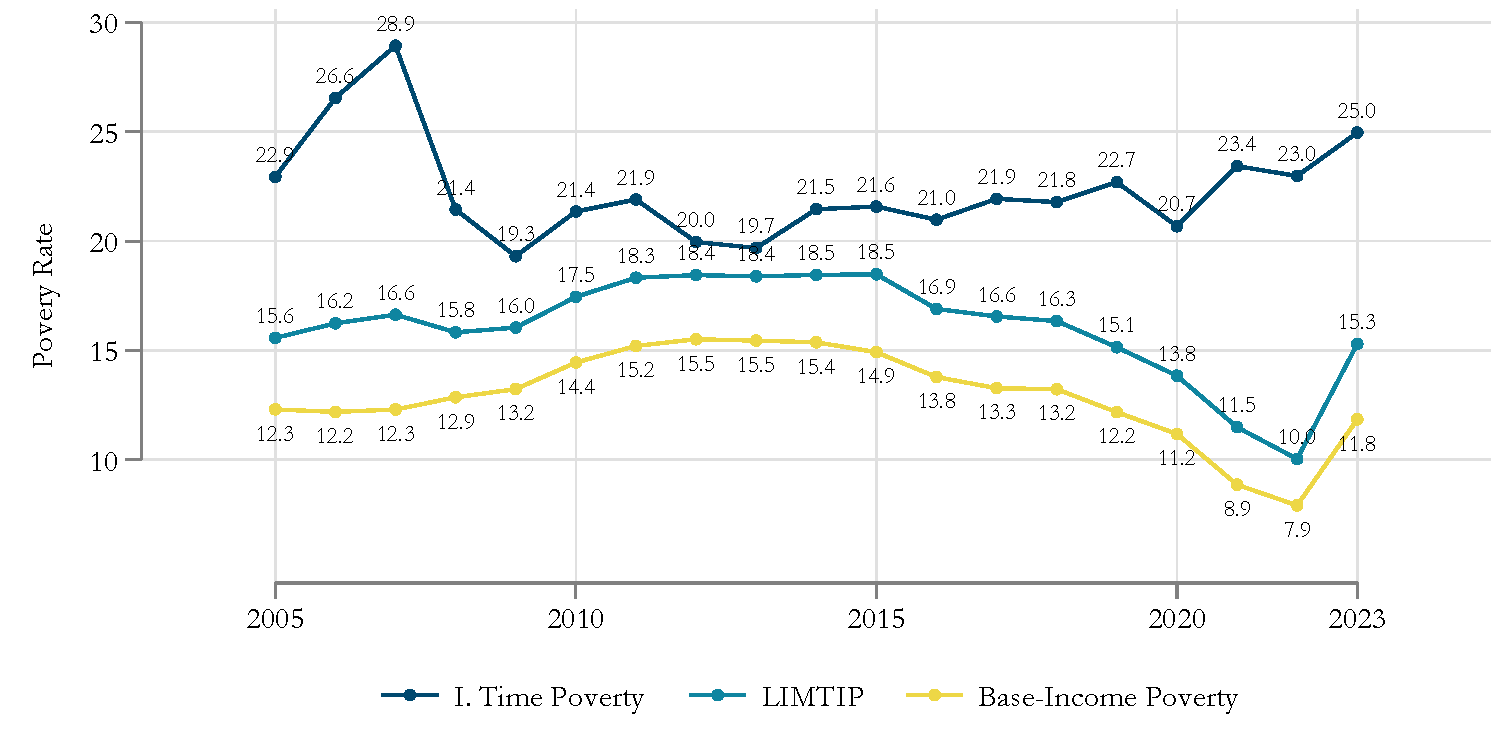
\includegraphics{resources/trend.pdf}

}

\caption{\label{fig-trend}Trends of Time, Income and Limtip Poverty in
the U.S.}

\end{figure}%

\section{Identifying the Problem}\label{sec-problem}

One of the strategies that could help reducing the problem of time
poverty, and thereby the incidence of hidden poor, is the redistribution
of household production responsibilities across all capable members in
the household. At best, household members with time surpluses could take
on more household responsabilities, reducing the burden of those with
time deficits. At worst, the redistribution could make the time deficits
more equal among the household members, even if the household remains
time poor.

Before we start analyzing the potential that redistribution could have
in reducing time poverty, we must first identify the households where
redistribution is possible and desirable. Specifically, we exclude from
the analysis households that are not time poor, even if such households
could potentially benefit from redistribution, reducing the gaps of time
surpluses among household members. From the sample of individuals living
in a time poor household we classify them into 5 different groups:

\begin{itemize}
\tightlist
\item
  Single: These are time poor individuals that live in a household where
  they are the only working-age person. In this case, redistribution is
  not possible, and thus are excluded from the analysis.
\item
  Time Poor living in H. Type I: These are time poor individuals who
  live in households where all working-age members are time poor. While
  redistribution is possible, and may help in reducing the time deficits
  of individuals, and even allow some to transition out of time poverty,
  the household will remain time poor in any redistributional scenario.
\item
  Time Poor living in H. Type II: These are time poor individuals who
  live in households where there are non-time poor individuals. However,
  the combined time surpluses is insufficient to lift the household out
  of time poverty.
\item
  Time Poor living in H. Type III: These are time poor individuals who
  live in households where there is enough time surplus to lift the
  household out of time poverty. Redistribution in these households can
  lift all working members of the household out of time poverty.
\item
  Non Time poor living in a time poor household: This last group
  consists of individuals with time surpluses living in a time poor
  household. The goal of the redistribution scenarios is to allocate
  household responsabilities in such a way that this invididuals can
  help lift other household members out of time poverty. However, it is
  also possible that some of these individuals may end up experiencing
  time poverty in the redistribution scenarios.
\end{itemize}

Figure~\ref{fig-composition} provides a visual representation of the
classification of individuals living in time poor households. As it can
be observed, across years, about 40\% of individuals were living in a
time poor household. While this share shows a sharp increase between
2005 and 2007, it has remained stable from 2008 onwards, with a small
increase across years. There is an additional 4-5\% of individuals who
are time poor but redistribution is not possible. From the rest, about
15\% of individuals constitute our main group of analysis, i.e., those
living in households where redistribution is possible and some
individuals could benefit from it. The remaining 20\% are individuals
who are not time poor but live in a time poor household.

\begin{figure}

\centering{

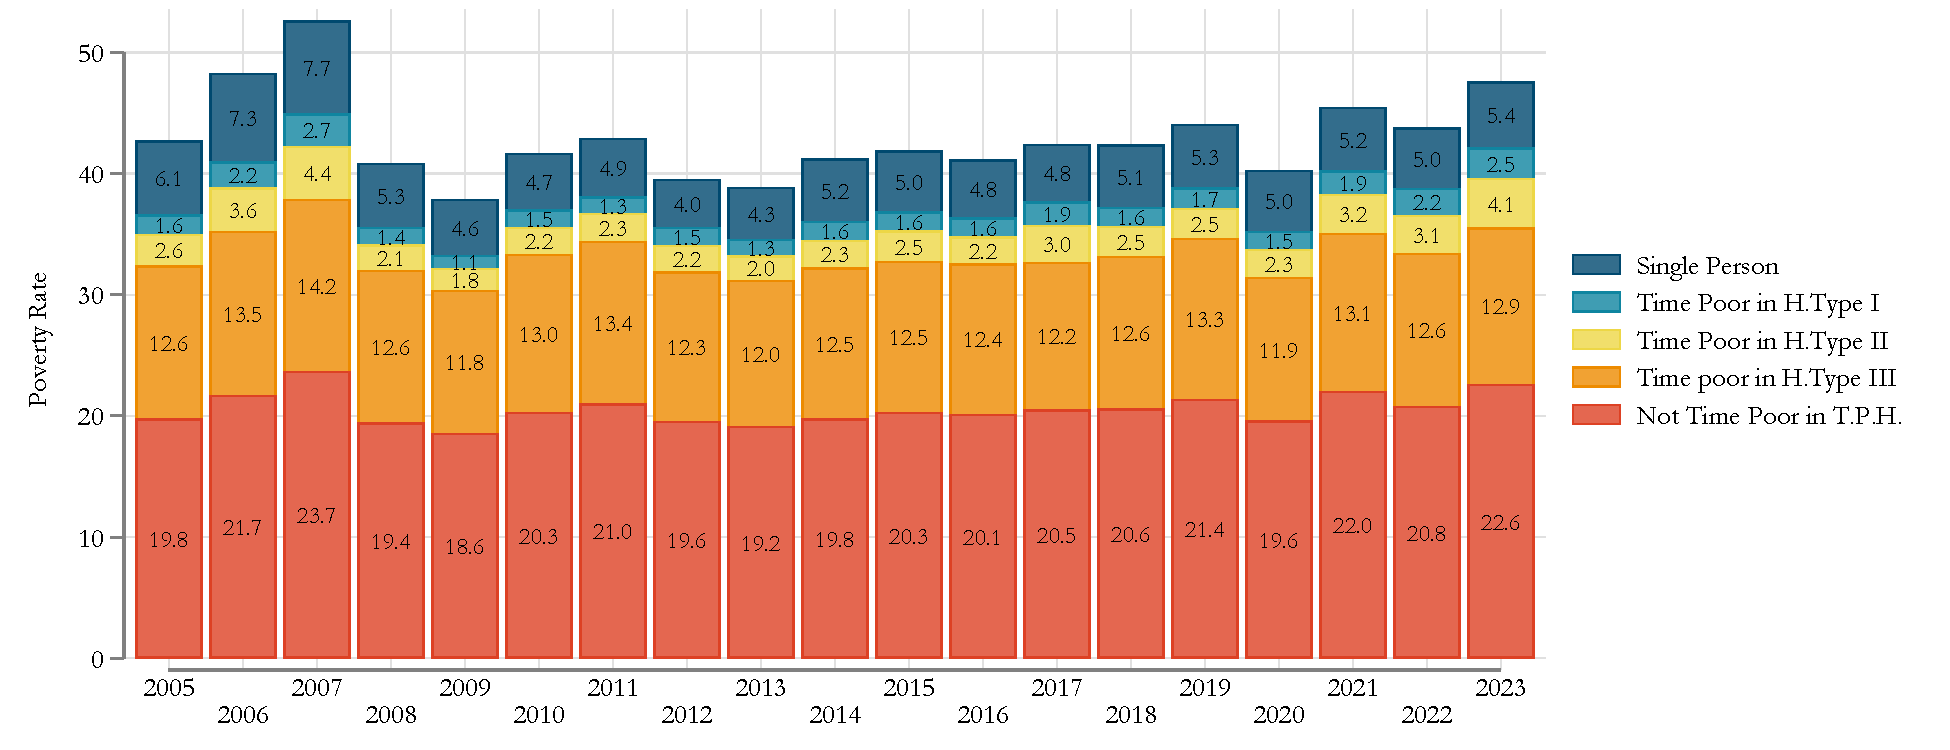
\includegraphics{resources/tpov_type.pdf}

\footnotesize 

\begin{flushleft}Note: T.P.H.= Time Poor Household, H.Type I : All working age members are time poor, H.Type II: There are Non-time poor individuals Living in the HH, but time surplus is insufficient to Lift HH out of Time poverty, H.Type III: There is enough time surplus to lift HH out of time poverty.\end{flushleft}

}

\caption{\label{fig-composition}Time Poverty classification, across
time}

\end{figure}%

In the next section, we discuss three redistribution scenarios where
household responsabilities could be redistributed across working-age
members, under different criteria. Nevertheless, we should keep in mind
that we will only be analyzing the impact of redistribution on time poor
households with at least 2 working-age members.

\section{Redistribution Scenarios}\label{redistribution-scenarios}

\begin{itemize}
\item
  Here we would describe the three redistribution scenarios we have
  developed. This would be ``realistic'' scenarios.
\item
  Describe the scenarios and the assumptions behind them.
\end{itemize}

Intrahousehold redistribution can potentially reduce time deficits. We
construct three redistrubution scenarios based on different guiding
principles. The extent of the reduction would depend on the principle
that we use in distributing household responsibilities among the
members. First, we use the simple egalitarianism principle that involves
an equal division of total household productiom time among all working
age members. Second, we redistribute conditional on the available time
people have. In the thord scenario, we redsitribute based on the
opportunity cost of time for people.

xxxx In the next section, we outline the methods used for implementing
the principles in our data, with the detailed explanation of some
aspects below:

\subsection{Distribution Rules for Household
Production}\label{distribution-rules-for-household-production}

Alternative values of \(\alpha_{ij}\) indicate how household production
requirements, net of the portion met by household members that are not
of working age or are physically unable to take on more work, are shared
between working-age persons in the household. Below we discuss the three
principles.

\subsubsection{1. Equal Shares Scenario}\label{equal-shares-scenario}

The procedure for the equal shares scenario is relatively simple. Recall
that the shares of those in the redistribution simulation in this
scenario are simply:

As before, denoting the number of working-age persons in household \(j\)
as \(I^j\), we can express the rule as:

\begin{equation}\phantomsection\label{eq-r1}{\alpha_{ij}^E= 1/I_j*(1-\alpha_{j}^{nw'})
}\end{equation}

We need to count how many people are in the redistribution simulation in
each household and then assign them the appropriate fraction (1 for
households with one person in the simulation, 1⁄2 for households with
two people in the simulation, and so on) and apply that fraction to the
redistributable share of required household production time.

\subsubsection{2. Time Available Scenario (WIP
editing)}\label{time-available-scenario-wip-editing}

The time available scenario is based on equity such that the
redistrubted shares are based on the time that is available after
setting aside the time for personal maintenance requirements and income
generation. In other words, the household members should split up the
required household production time based on the time each one has
available, i.e based on an equity criteria. The time available
(\(Z_{ij}\))) is defined as the time left over after the minimum
personal maintenance and time spent on income generation (including
commuting time) have been subtracted from the total weekly hours. To
calculate the shares for each individual based on this principle, we
first calculate the time available for each individual, then add up the
total among the household for those individuals that have positive time
available. We then divide each individual's time available by the total
and apply that fraction to the redistributable share of household
production time. For those individuals that have negative time available
we set their shares to zero in this simulation.

\subsubsection{3. Opportunity costs}\label{opportunity-costs}

The third possibility is based on the idea of opportunity costs along
marginalist lines. The sharing rule depends on the relative actual
(potential) wage. For example, if there are only two working-age adults,
say husband and wife, and if the husband's wage is twice as much as the
wife, the wife's share would be two-thirds and the husband's share would
be one-third. We use the actual or shadow wage for the employed and the
potential wage for the nonemployed. Redistribution takes place based on
the following equation:

First, we imputed wages for all of those not currently working for pay.
In order to do this, we used a two-stage Heckman selection model
(Heckman 1979), also known as the Heckit procedure, which we outline
below. Once done, we used the imputed wages of those that are not
currently working for pay and the actual wages of those that are working
to divide up the redistributable share of required household production:

\begin{equation}\phantomsection\label{eq-r3}{\alpha_{ij}^O= (1/{I_j-1})*(1-w_{ij}/w_{ij} ) (1-\alpha_{j}^{nw'})
}\end{equation}

As the share of required household production needs to be inversely
proportional to the individual's share of the sum of wages, we subtract
their share of this sum from one. To ensure that the resulting shares
sum up to unity, we divide by the number of individuals in the
simulation minus one. We then apply this share to the redistributable
share of required household production as in previous steps. In order to
impute wages for those not currently employed for wages, we first impute
the likeliest industry and occupation for each individual using a
multinomial probit procedure. Industry and occupation are regressed on
age, age squared, sex, race, education, and geographic region on all
those in the working age population (18-64). The likelihood for each
industry and occupation is then predicted for everyone, using the
results of the multinomial probit. Then each individual not currently
working for wages is assigned the industry and occupation corresponding
to the xxxx/ largest predicted likelihoods for that individual.

Next, we move on to the first stage of the Heckit procedure, a probit
estimation of a dummy variable for being employed in wage work (paid):

\begin{equation}\phantomsection\label{eq-probit}{P(paid=1|X)=F(X* \beta)
}\end{equation}

where F is the cumulative density function of a normal distribution. The
vector of explanatory variables, 𝑋, comprises the individual's age, sex,
race, disability, number of kids across age groups (0 to 5, 6 to 14,
15-17), presence of spouse and spouse's age, education and employment
status education. The regression is run on the universe of all eligible
adults separately by age (divided into four categories: 18 to 30 years
old; 31 to 45 years old; and 46 to 64 years old) and sex. The Mills
ratio, 𝜆, is calculated for all individuals using the results of the
first stage regression:

where 𝑓 and 𝐹 are, respectively, the probability and cumulative density
function of a normal distribution, and 𝛽􏱞 is the vector of estimated
coefficients from the probit model. The second stage is an ordinary
least squares (OLS) estimate of the log of hourly wage:

\[lnw= (\gamma_2*Z^w) + (\theta_2 * \lambda) +
\]

This regression is run only on those that are actually employed for pay
(!FRA). The vector of explanatory variables, {[}{]}, includes age, sex,
race, education, geographical region, disability, industry, occupation,
presence of spouse, spouse's employment status, and, finally, λ, the
Mills ratio calculated in the first stage. Inclusion of the Mills ratio
corrects for the selection bias induced by limiting the regression to
those in paid employment. The imputed log of wage is predicted for those
not working for wages from the results of the regression, with industry
and occupation replaced by the industries and occupations assigned in
the previous step.

Describe our procedue : 2 stages

We simulate each of these principles of redistribution and recalculate
individual and household time and income poverty using the LIMTP
framework described above.

\begin{itemize}
\tightlist
\item
  Next, we provide an assessment of the different principles in terms of
  how far they improve the position of women and how much such
  improvements are congruent with the betterment of the economic
  well-being of their families. In the subsequent section, we compare
  and contrast the joint distribution of time and income poverty among
  families and individuals that would result from each principle.
\end{itemize}

\section{Results}\label{results}

As described in the previous section, we consider three scenarios to
analyze the impact that redistribution could have on time poverty,
focusing on individuals living in time poor households with at least two
working-age members. In this section, we present the results of the
redistribution scenarios and discuss the implications for time poverty
and the incidence of hidden poor. Since most of the results acrosstime
(see online appendix) are similar, we focus on providing results that
average the impacts of redistribution across all years.

\subsection{Redistribution Scenarios and Time Poverty: General
Results}\label{redistribution-scenarios-and-time-poverty-general-results}

Based on the imputed data, and considering people in working age only,
55 out of 100 individuals that live in time poor households are not time
poor themselves. 4.6 live in households where everyone is time poor,

\begin{figure}

\centering{

\begin{figure}[H]

\begin{minipage}{0.50\linewidth}

\centering{

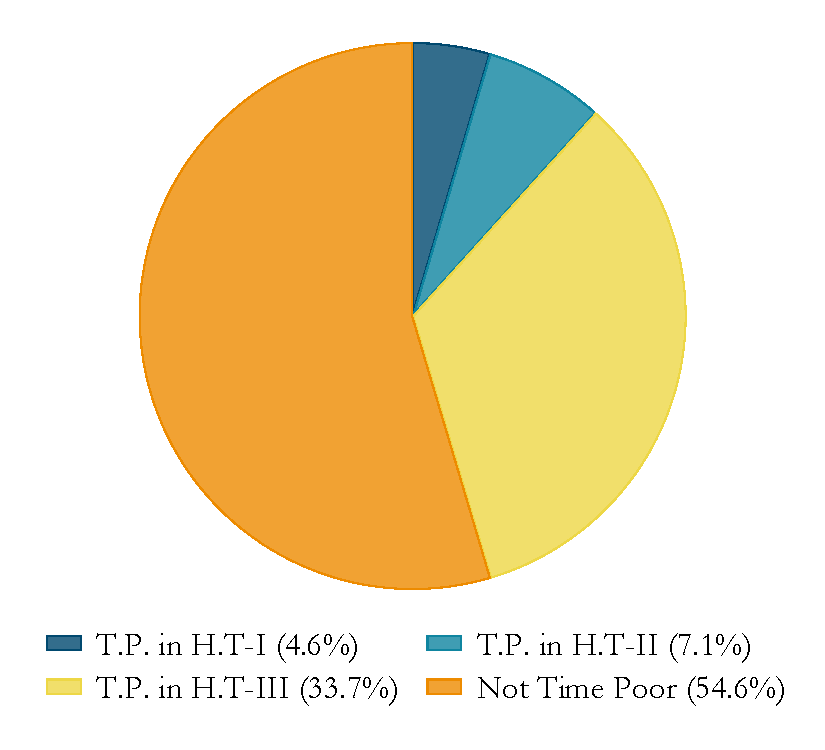
\includegraphics{resources/ind_dist.pdf}

}

\subcaption{\label{fig-dista}Individuals}

\end{minipage}%
%
\begin{minipage}{0.50\linewidth}

\centering{

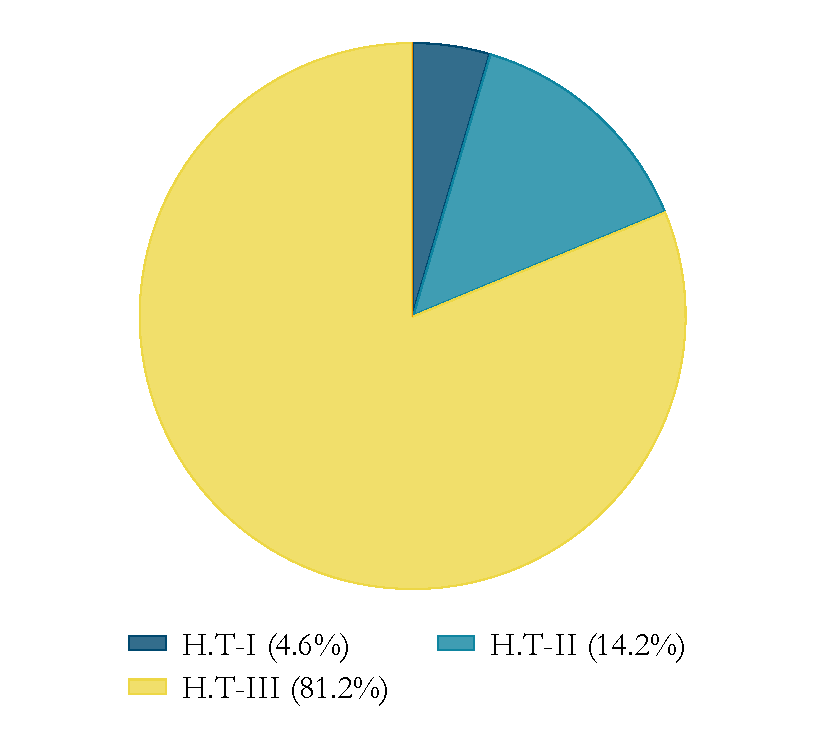
\includegraphics{resources/hh_dist.pdf}

}

\subcaption{\label{fig-distb}Households}

\end{minipage}%

\end{figure}%

\footnotesize 

\begin{flushleft}Note: H.Type I : All working age members are time poor, H.Type II: There are Non-time poor individuals Living in the HH, but time surplus is insufficient to Lift HH out of Time poverty, H.Type III: There is enough time surplus to lift HH out of time poverty.\end{flushleft}

}

\caption{\label{fig-dist}Distribution of individuals by type}

\end{figure}%

To understand the impact of the diferent redistribution scenarios on
this groups, we will focus on transition probabilities. Thus, for those
out of poverty, our statistic of interest would be the likelihood that
they fall back into poverty, and for those in poverty, the likelihood
that they transition out of poverty.

\begin{figure}

\centering{

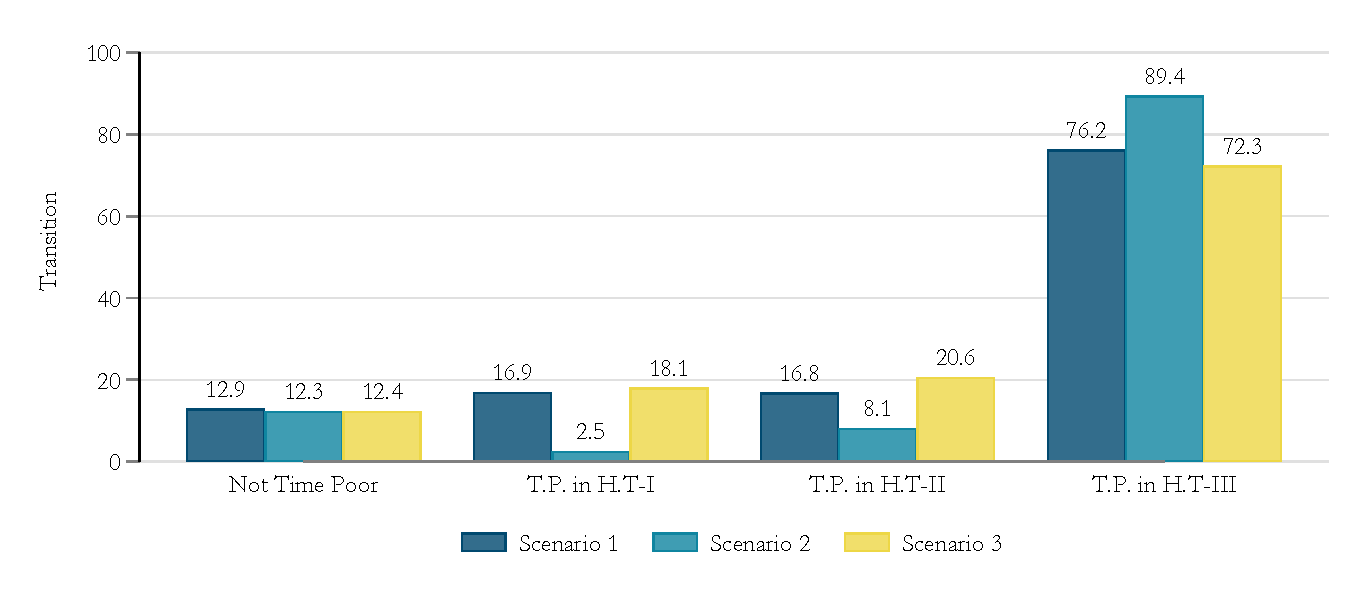
\includegraphics{resources/trans1.pdf}

}

\caption{\label{fig-transition1}Transition probabilities by
Redistribution Scenario}

\end{figure}%

\begin{figure}

\centering{

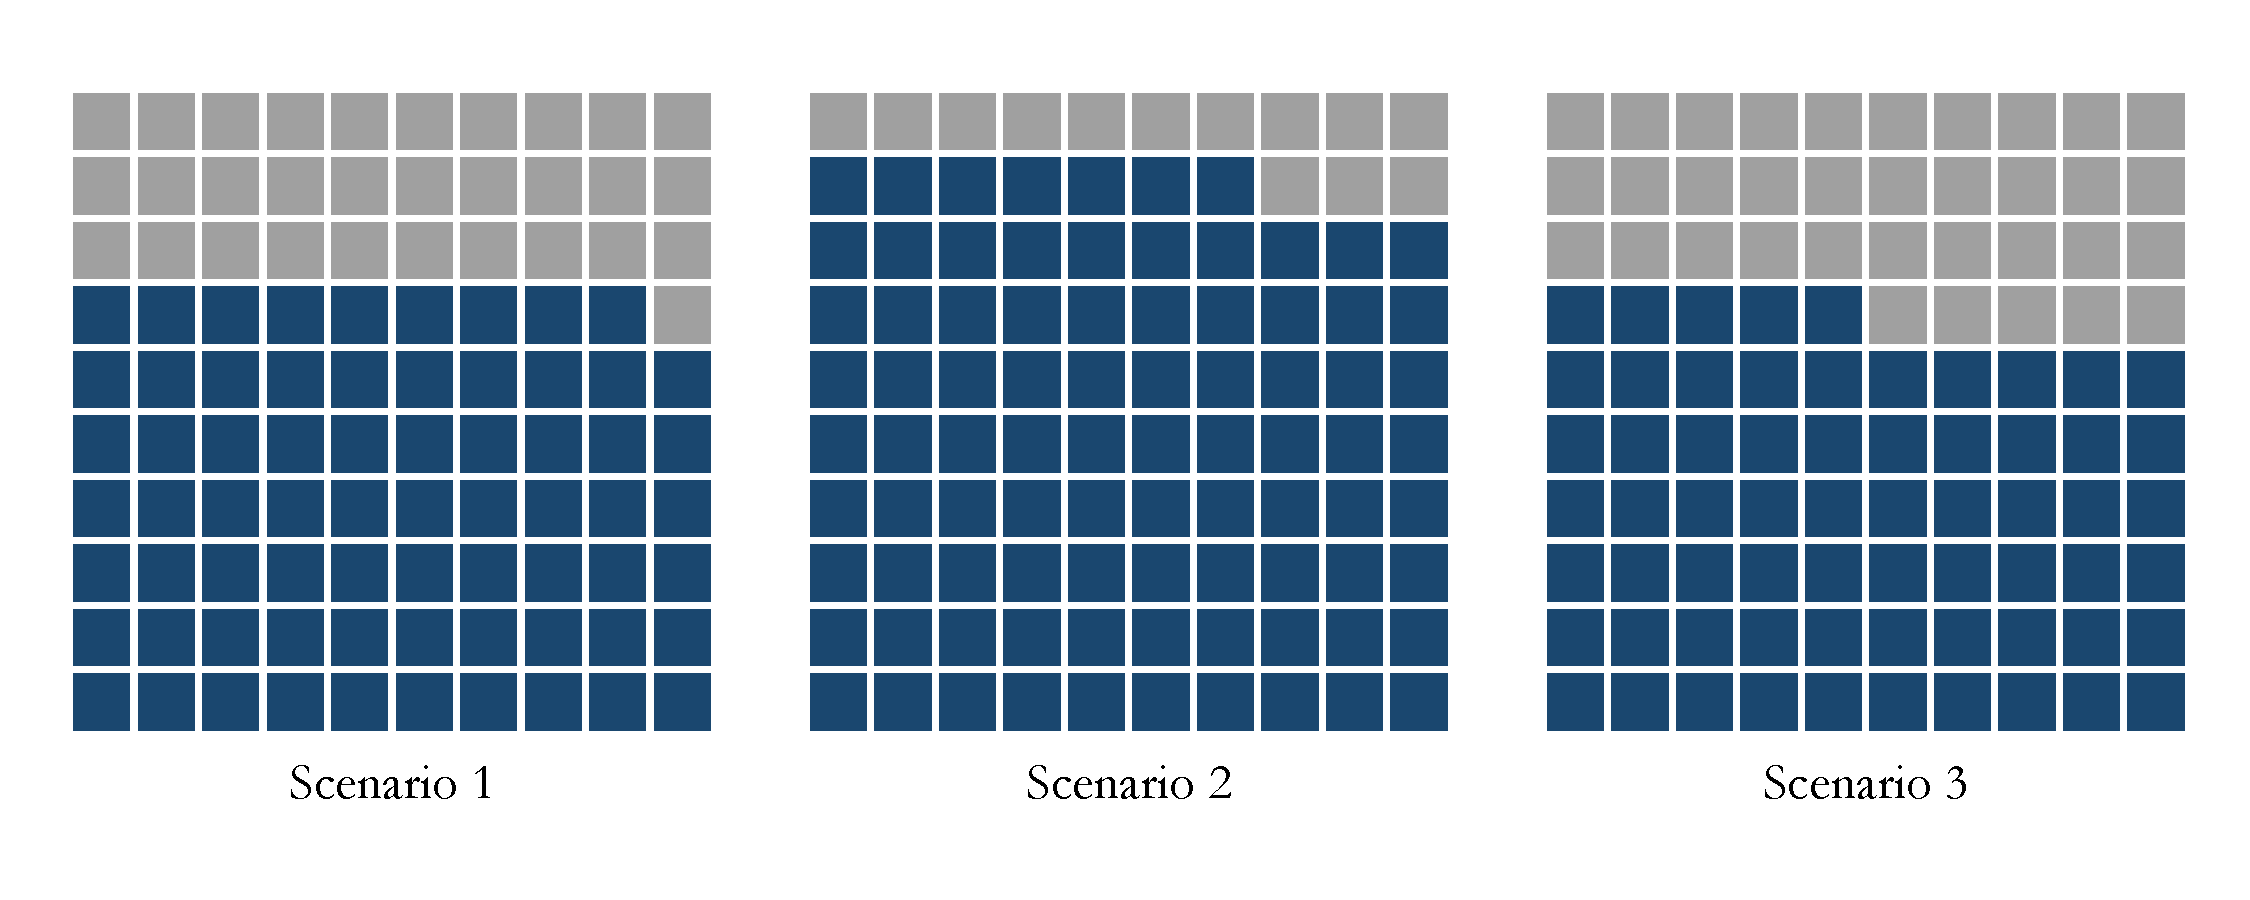
\includegraphics{resources/hhtrans.pdf}

}

\caption{\label{fig-transition2}Transition probabilities for households}

\end{figure}%

Of course, the scenarios also have implications in terms of time poverty
gap (time deficits). As shown in

\begin{figure}

\centering{

Plot on time Deficits: Across Different Scenarios

}

\caption{\label{fig-transition}-----------------+----------------------------------------
Not Time Poor \textbar{} 0 -.7191797 -.5483149 -.7216919 Lives in T-I h
\textbar{} -10.68127 -11.5814 -10.72205 -11.62268 Lives in T-II h
\textbar{} -20.32136 -9.095953 -5.58591 -10.04065 Lives in T-III h
\textbar{} -10.45076 -2.27825 -.4266873 -2.103088
-----------------+---------------------------------------- Perhaps
Mandoline plot}

\end{figure}%

\subsection{Redistribution Scenarios and Time Poverty:
Heterogeneity}\label{redistribution-scenarios-and-time-poverty-heterogeneity}

In this section, we present the results of the redistribution scenarios
analyzing the impact on time poverty across different demographic
groups.

Perhaps Mandoline plot for all scenarios by group: Three groups. We only
see Individuals Here

\begin{figure}

\centering{

\captionsetup{labelsep=none}Transition probabilities across types
individuals, by Group

}

\caption{\label{fig-tran_by_group1}}

\end{figure}%

\begin{figure}

\centering{

\captionsetup{labelsep=none}Deficits by group

}

\caption{\label{fig-tran_by_group1}}

\end{figure}%

\section{Policy implications}\label{policy-implications}

\section{Conclusion}\label{conclusion}

\section*{References}\label{sec-ref}
\addcontentsline{toc}{section}{References}

\phantomsection\label{refs}
\begin{CSLReferences}{1}{0}
\bibitem[\citeproctext]{ref-berik2009}
Berik, G., Rodgers, Y. van der M., and Seguino, S. (2009). Feminist
{Economics} of {Inequality}, {Development}, and {Growth}. \emph{Feminist
Economics}, \emph{15}(3), 1--33.
\url{https://ezprox.bard.edu/login?url=https://search.ebscohost.com/login.aspx?direct=true&db=ecn&AN=1063369&site=eds-live&scope=site}

\bibitem[\citeproctext]{ref-hundt1996}
Bruyn-Hundt, M. (1996). Scenarios for a redistribution of unpaid work in
the netherlands. \emph{Feminist Economics}, \emph{2}(3), 129--133.
\url{https://doi.org/10.1080/13545709610001707826}

\bibitem[\citeproctext]{ref-duflo2012}
Duflo, E. (2012). Women {Empowerment} and {Economic} {Development}.
\emph{Journal of Economic Literature}, \emph{50}(4), 1051--1079.
\url{https://doi.org/10.1257/jel.50.4.1051}

\bibitem[\citeproctext]{ref-elson2017}
Elso, D. (2017). \emph{Recognize, {Reduce}, and {Redistribute} {Unpaid}
{Care} {Work}: {How} to {Close} the {Gender} {Gap}}.
\url{https://doi.org/10.1177/1095796017700135}

\bibitem[\citeproctext]{ref-elson2009}
Elson, D. (2009). Gender {Equality} and {Economic} {Growth} in the
{World} {Bank} {World} {Development} {Report} 2006. \emph{Feminist
Economics}, \emph{15}(3), 35--59.
\url{https://doi.org/10.1080/13545700902964303}

\bibitem[\citeproctext]{ref-valeria2016}
Esquivel, V. (2016). Power and the {Sustainable} {Development} {Goals}:
A feminist analysis. \emph{Gender \& Development}, \emph{24}(1), 9--23.
\url{https://doi.org/10.1080/13552074.2016.1147872}

\bibitem[\citeproctext]{ref-hess2020}
Hess, Cynthia, Ahmed, T., and Hayes, J. (2020). \emph{Providing {Unpaid}
{Household} and {Care} {Work} in the {United} {States}: {Uncovering}
{Inequality}}.

\bibitem[\citeproctext]{ref-malik2018}
Malik, R., Hamm, K., Schochet, L., Novoa, C., Workman, S., and
Jessen-Howard, S. (2018). America's {Child} {Care} {Deserts} in 2018.
\emph{Center for American Progress}.
\url{https://www.americanprogress.org/article/americas-child-care-deserts-2018/}

\bibitem[\citeproctext]{ref-oecd2020}
OECD. (2020). \emph{Early learning and child well-being in the united
states} (p. 124).
https://doi.org/\url{https://doi.org/https://doi.org/10.1787/198d8c99-en}

\end{CSLReferences}



\end{document}
